\hone{Allgemeines}
\sectionauthor{Julian Kusternigg}

\htwo{Einführung}

% TODO:
% Passiv vermeiden?
% Beistrichsetzung!!
Das "Zentrale, Einheitliche LehrraumInformationsAuslesystem", kurz ZELIA, ist vereinfacht gesagt ein Programm, mit dem man Informationen von Lehrräumen abfragen und verändern kann. Das Ziel von \ZELIA\ ist in Schulen verwendet zu werden, um schnell Infos über Räume zu erlangen, ohne sich an Lehrer*innen wenden zu müssen. Da \mbox{ZELIA} im "Schulzentrum Ungargasse" entwickelt wurde, beziehen sich Tests und Beispiele oft auf dieses. Die Anwendung des Programmes ist jedoch ortsunabhängig, da die einzige Voraussetzung zur Verwendung eine gültige Raumnummer ist. Somit könnte man \ZELIA\ auch in anderen Schulen ausrollen und verwenden. 

\begin{figure}[H]
    \centering
    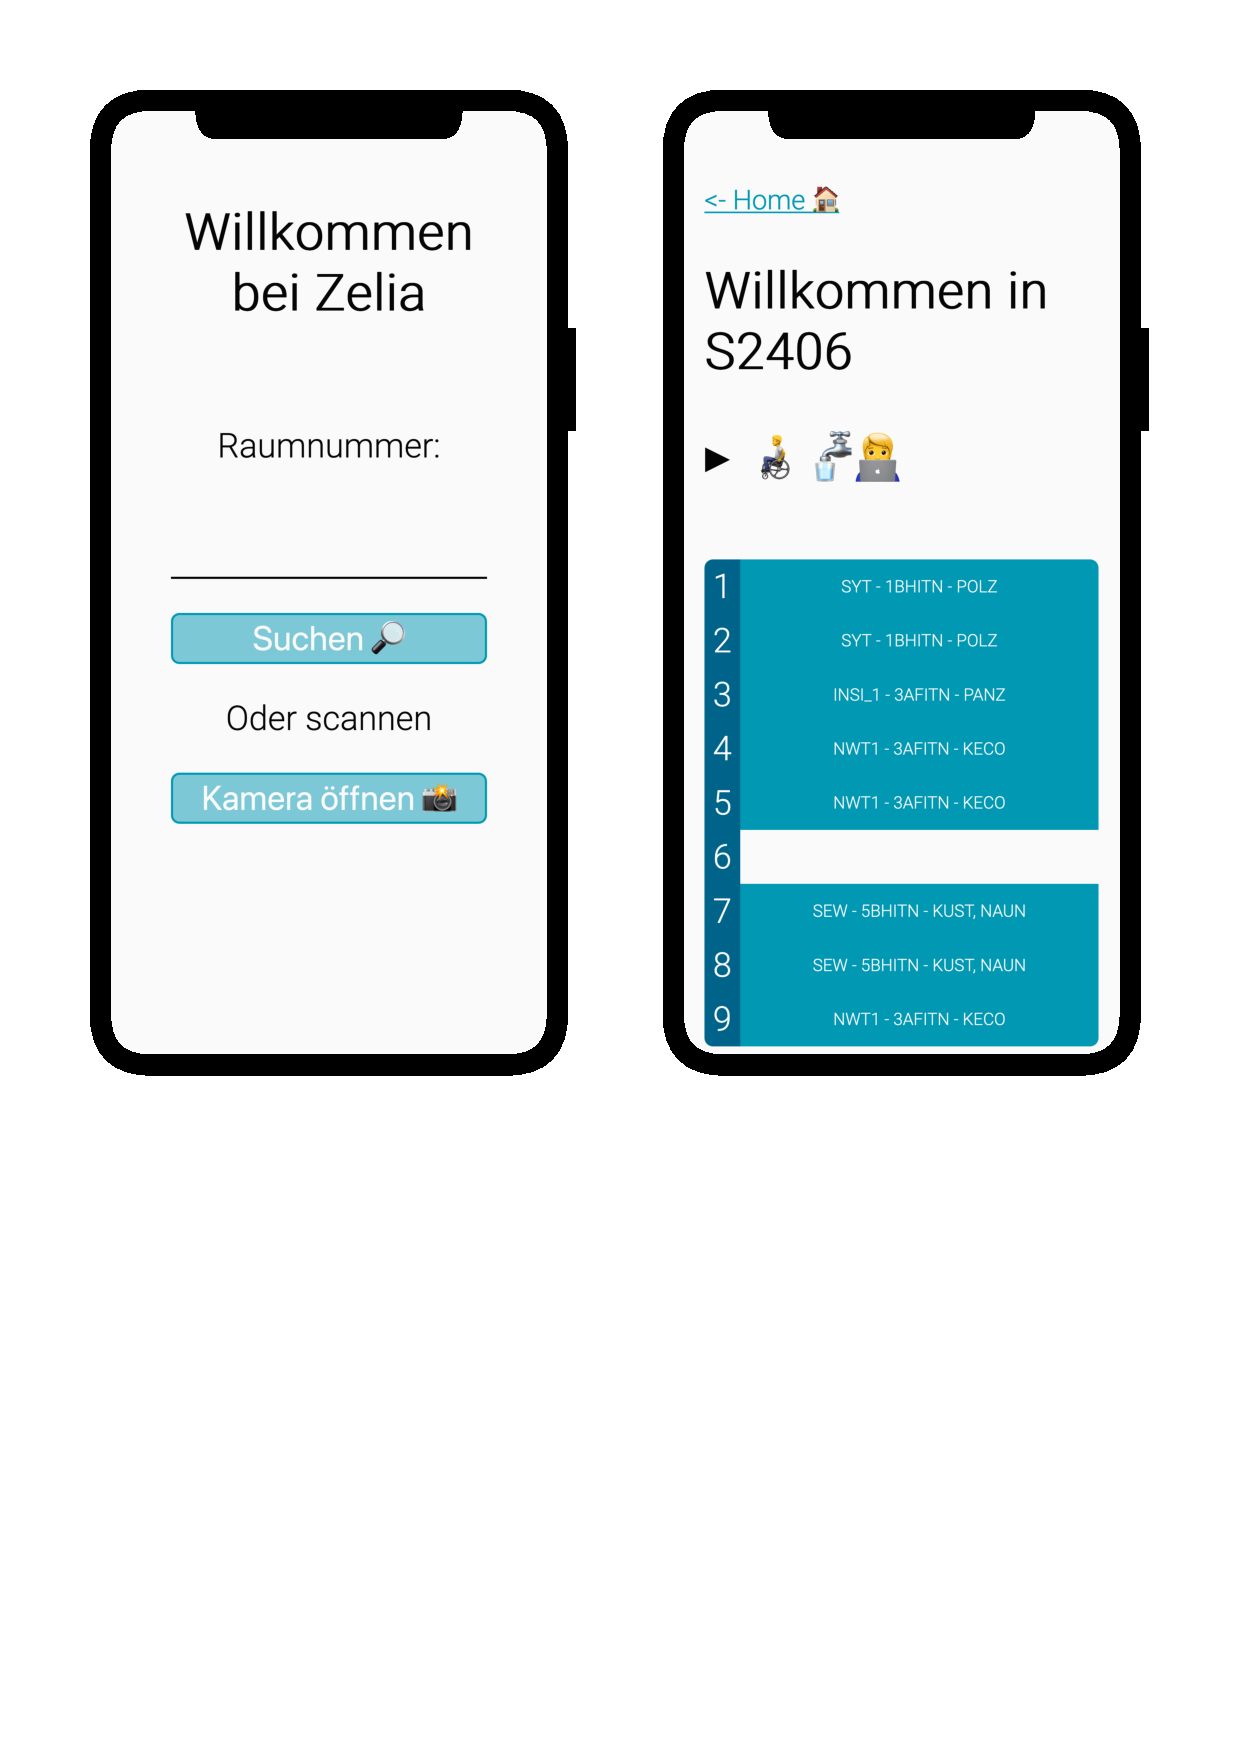
\includegraphics[width=120mm]{media/Intro/frontend_mobile.svg.pdf}
    \caption{Mobilansicht der Web-Applikation}
\end{figure}

Die Benutzeroberfläche von \ZELIA\ läuft als Web-Applikation. Das bedeutet, dass man nur einen Browser braucht mit dem man die Seite aufrufen und verwenden kann. Das Backend läuft in Docker-Containern, welche es möglich machen, den Server unabhängig von der verwendeten Hardware zu starten (siehe Kapitel Containertechnologie und Docker in Kapitel \ref{sec:ContainerAndDocker}).

Informationen über einen Raum kann man mit der jeweiligen Raumnummer einfach in der Web-Applikation abfragen. Bei diesen Infos handelt es sich zum einen um Standarddaten eines Raumes. Beispiele dafür wären, die Anzahl von Plätzen und Computern in einem Raum oder welche Arten von Tafeln sich in diesem befinden. Zum anderen werden die Raumstundenpläne von WebUntis abgefragt, damit man immer den aktuellen Stundenplan sehen kann.

Neben dem Abfragen von Rauminformationen, kann man mit \ZELIA\ auch Anmerkungen zu Räumen erstellen. Dadurch kann man Defekte oder Mängel in Räumen melden. Zusätzlich kann man Räume buchen, falls diese frei sind und für Nachhilfe oder andere Zwecke verwenden. Diese Meldungen und Buchungen können von "Administratoren" in der Web-Anwendung angesehen und auch abgearbeitet werden. Bei diesen Administratorbenutzern handelt es sich um Lehrer*innen, die sich um beliebige Räume kümmern. Dadurch können entweder bestimmte Klassenräume von bestimmten Lehrern, sprich Administratoren, verwaltet werden oder alle Räume werden von einer Person verwaltet.

Um eine Meldung oder Buchung zu tätigen, muss man eine E-Mail-Adresse von sich selbst angeben. Im Fall von \ZELIA\ im Schulzentrum Ungargasse eine Schul-Mail-Adresse, die alle Schüler*innen haben. An die angegebene E-Mail-Adressen wird ein Bestätigungslink geschickt und erst wenn dieser aufgerufen wird, ist die Anfrage genehmigt. Dadurch wird verhindert, dass man sich einen Account anlegen muss um Meldungen zu tätigen. Trotzdem kann man nachvollziehen, welche Schüler*innen Defekte gemeldet haben. Dieses Konzept wird bei \ZELIA\ auch deshalb verwendet, da sich vermutlich niemand einen Account anlegen möchte oder mühsam mit einem vorgegebenen Benutzer anmelden will. Die Schul-Mail-Adressen, die alle besitzen, sind in diesem Fall viel komfortabler. Es kann passieren, dass Schüler*innen sich einen Spaß erlauben und nicht ihre eigene Mail-Adresse angeben. Dadurch würde irgendjemand eine Mail bekommen, die nicht gewünscht ist. Das ist aber kein Problem das es nur mit \ZELIA\ gibt, denn es können sowieso alle Schüler*innen sich gegenseitig so viele Mails schicken wie sie wollen. Als Lösung dafür könnte man einen eigenen Ordner für alle \ZELIA\ Bestätigungen einrichten oder man könnte limitieren, dass nur eine bestimmte Anzahl an Meldungen pro Zeitintervall gemacht werden darf. Wenn nun eine Buchung akzeptiert oder abgelehnt wird, bekommt man eine Mail geschickt, in der ein kurzer Informationstext steht und ob man den Raum benutzen darf oder ob die Anfrage abgelehnt wurde.

ZELIA ist spezifisch für Schulen entwickelt und somit besteht die Zielgruppe vor allem aus Schüler*innen und Lehrer*innen, die täglich in mehreren Lehrräumen unterwegs sind. Für diese ist es praktisch zu sehen in welchem Raum sie später vielleicht sein werden und welche technischen Mittel dort zur Verfügung stehen. Aber auch für Besucher*innen einer Schule, zum Beispiel an einem "Tag der offenen Tür", könnte \ZELIA\ von Nutzen sein. So könnte man selbst, ohne Begleitung, durch die Schule gehen und Informationen über Räume und \zb\ Projekte in diesen, erfahren.

\begin{minipage}{\textwidth}
    Aufteilen kann man \ZELIA\ in drei Teile: 
    \begin{itemize}
        \item Den Server
        \item Die Datenbank
        \item Den Client
    \end{itemize}
    Jeder dieser Teile ist in sich geschlossen, einzeln geplant und implementiert worden.
\end{minipage}

\begin{figure}[H]
    \centering
    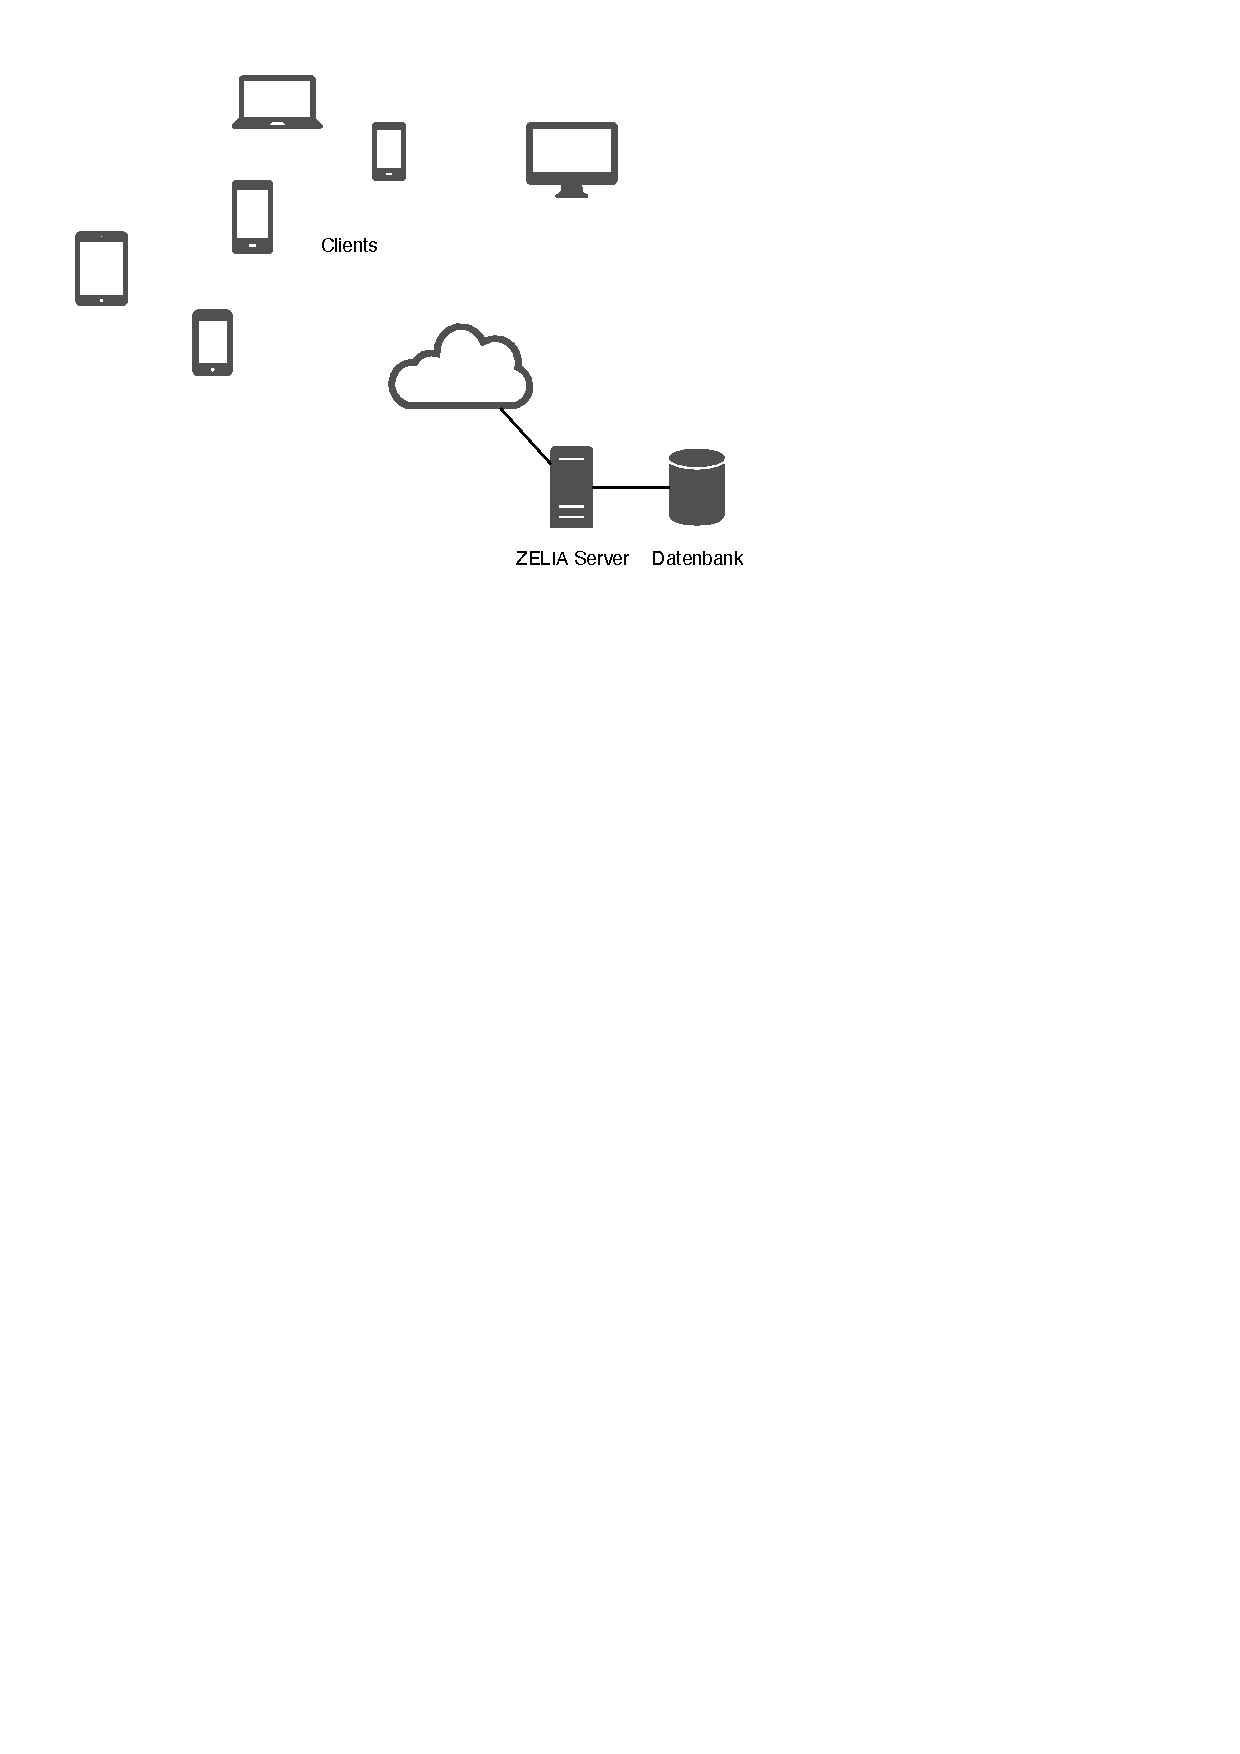
\includegraphics[width=120mm]{./media/Intro/client_server_arch.svg.pdf}
    \caption{Server-Client-Verbindung}
\end{figure}

\htwo{Server}

Der ZELIA-Server ist der Hauptteil von ZELIA. Er sammelt und stellt alle Daten zur Verfügung, welche benötigt werden, um die Software auf den Endgeräten, also den Clients, darzustellen. Dafür wird der Server nochmal in drei Teile unterteilt.

\begin{itemize}
    \item Der erste und wichtigste Teil ist die Schnittstelle für die Endgeräte, genannt ZELIA-API ("Application Programming Interface"). Über diese Schnittstelle fragt das Client-Programm Informationen über Räume ab oder sendet Meldungs- und Buchungsanfragen aus.
    \item Der zweite Teil ist die Schnittstelle zwischen Server und Datenbank. Primär werden aus der Datenbank Informationen über Räume abgefragt. Auch andere Daten wie Administratorbenutzer, um Meldungen und Buchungen zu verwalten, stehen in der Datenbank zur Verfügung. 
    \item Der dritte Teil kümmert sich um die Abfragen von WebUntis, um Zugriff auf aktuelle Stundenpläne jeweiliger Räume zu bekommen.
\end{itemize}

Während das Backend für den Client nur ein Server ist, besteht dieser eigentlich aus mehreren Docker-Containern. Dadurch ist es möglich, die Datenbank und die ZELIA-API am selben Server in sogenannten Containern laufen zu lassen. Ein großer Vorteil daran ist, dass man \ZELIA\ als gesamtes System starten und verwalten kann. Gerade in der Entwicklung ist das sehr wichtig, da somit auf jedem beliebigen Computer eine eigene \ZELIA\ Instanz gestartet werden kann. Für diese Container macht es keinen Unterschied, ob sie nebeneinander am selben Server laufen oder nicht. Sie sind miteinander über ein virtuelles Netz verbunden (mehr zu Containertechnologie und Docker in Kapitel \ref{sec:ContainerAndDocker}, Seite \pageref{sec:ContainerAndDocker})

\begin{figure}[H]
    \centering
    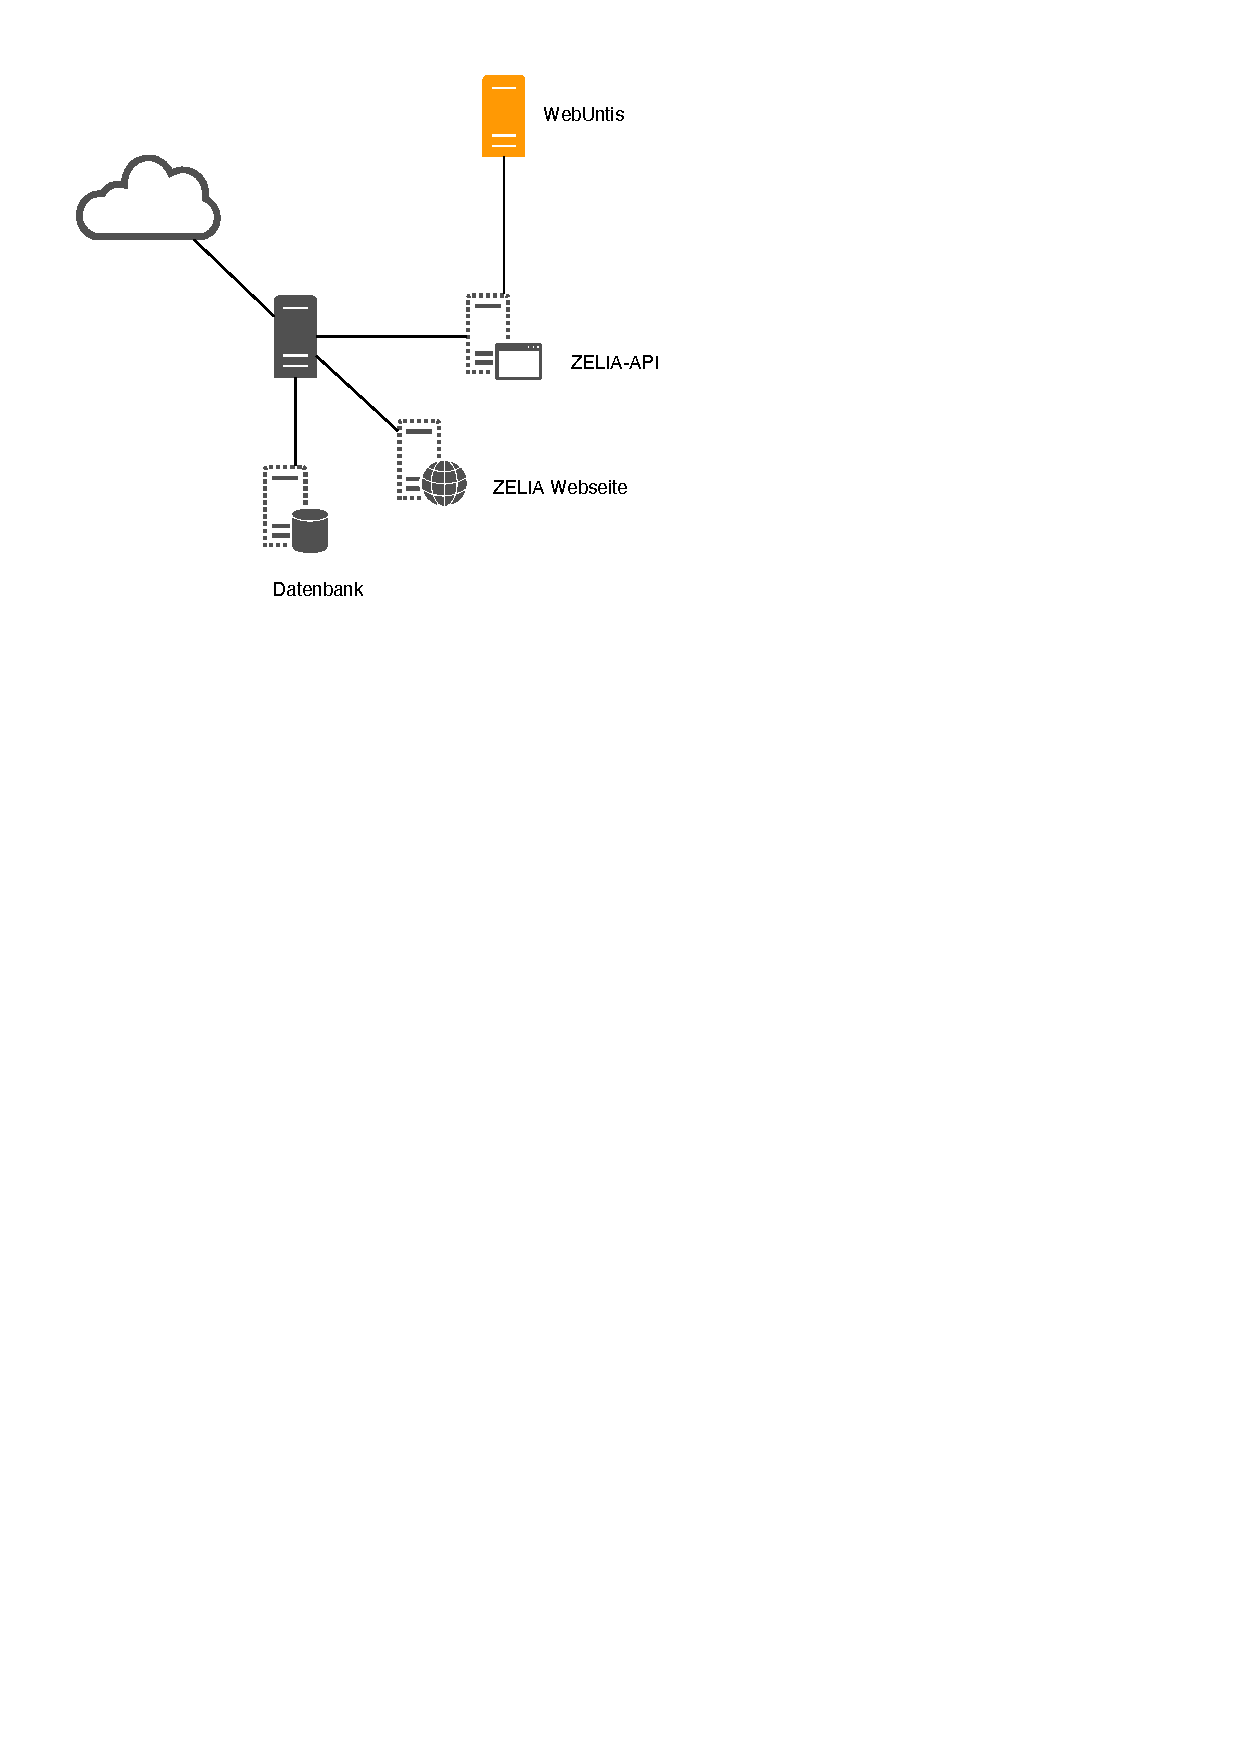
\includegraphics[width=120mm]{./media/Intro/server_arch.svg.pdf}
    \caption{Aufbau des ZELIA-Servers}
    \label{fig:server_arch}
\end{figure}

Der \ZELIA-API Server ist mittels NodeJS implementiert, ein Javascript-Framework, dies ermöglicht einfach mit dem Frontend zu kommunizieren. Außerdem gibt es viele vorgefertigte Pakete, um schnell ein stabiles Backend zu entwerfen. Statt Javascript wird bei \ZELIA\ allerdings TypeScript verwendet, welches aber in Javascript umgewandelt wird. Was genau TypeScript ist und warum es bei \ZELIA\ verwendet wird, ist in Kapitel TypeScript \ref{sec:TypeScript} (Seite \pageref{sec:TypeScript}) erläutert.

\htwo{Datenbank}

Die \ZELIA\ Datenbank ist physisch gesehen ein Teil des \ZELIA\ Servers (siehe Abbildung \ref{fig:server_arch}). Alle Informationen zu Räumen, wie die Anzahl von Plätzen oder Computern, werden in ihr gespeichert. Dort sind auch Meldungen und Buchungen von Räumen abgelegt, damit später darauf zurückgegriffen werden kann. Diese Meldungen und Buchungen können von Administratorbenutzern abgefragt werden. Diese Administratoren sind auch in der Datenbank gespeichert. Die Datenbank steht abgeschottet in einem privaten Netz, welches mittels Containertechnologien (siehe Kapitel Containertechnologie und Docker \ref{sec:ContainerAndDocker}) bewerkstelligt wird und kann nur über definierte Schnittstellen vom Server angesprochen und abgefragt werden. Verwendet wird die Datenbank "MariaDB" (siehe Kapitel MariaDB \ref{sec:MariaDB}). Am Datenbankteil des ZELIA-Servers wird "Sequelize" verwendet, um Abfragen zu machen (siehe Kapitel Sequelize \ref{sec:sequelize}).


\htwo{Client}

Damit \ZELIA\ einfach zu verwenden ist, baut der Client auf modernen Web-\linebreak Technologien auf. Somit ist der \ZELIA-Client eine Web-Anwendung,  die von jedem Gerät verwendet werden kann, egal ob Computer, Tablet oder Smartphone. Da \ZELIA\ mobil sein muss, ist die Web-Applikation so optimiert, dass sie auch auf leistungsschwächeren Geräten und Smartphones gut funktioniert. Das Frontend wurde mit Fokus auf eine einfache Verwendung auf Smartphones entwickelt, da es durch die Außenkameras dieser Endgeräte ein wichtiges Feature gibt. Normalerweise, also auf Geräten ohne Außenkamera, muss man die Raumnummer selbst eingeben, um die Informationen von einem Raum zu bekommen. Durch die Außenkamera von Smartphones gibt es allerdings die Möglichkeit Raumnummern, zum Beispiel von Türschildern, einzuscannen. 

Nachdem man auf der Startseite eine Raumnummer eingegeben hat, egal ob manuell oder gescannt, sieht man die jeweiligen Informationen eines Raumes. Wie schon erwähnt, gibt es auch die Möglichkeit Räume zu buchen oder Informationen über diese zu melden. Meldungen und Buchungen können im sogenannten "Admin Dashboard" angesehen und nach Relevanz gefiltert werden. Auf diese Administratorübersicht kann auch über die Web-Anwendung zugegriffen werden. Allerdings ist dafür ein gültiger Benutzername und Passwort eines Administrators, welcher in der Datenbank gespeichert ist, nötig.

Realisiert ist das Frontend von \ZELIA\ von Grund auf mit HTML5 und CSS3. Statt Javascript wird auch hier TypeScript verwendet, welches aber in normales vom Browser interpretierbares Javascript umgewandelt wird. 

Das Frontend läuft mit Ausnahme von der Bibliothek TesseractJS (siehe Kapitel Tesseract \ref{sec:tesseract}), welche verwendet wird um Text aus Bildern auszulesen, ohne fremde Bibliotheken. Dies wird benötigt um mit der Kamera eines Endgerätes Raumschilder einscannen zu können. Aus zwei Gründen wurden keine anderen Bibliotheken verwendet:
\begin{itemize}
    \item Bibliotheken, wie zum Beispiel Angular, sind für den Anwendungsfall an ZELIA sehr groß. Dadurch könnte die Webseite schnell zu komplex und langsam werden.
    \item Um herausfinden, wie man eine eigene einfache Bibliothek entwickeln kann, welche nicht nur für eine Anwendung konzipiert ist
\end{itemize}

Somit wurden zwei separate Teile entwickelt, auf denen das ZELIA-Client basiert. 
\begin{itemize}
    \item Ein Web-Komponentensystem, um den Inhalt der jeweiligen Seite anzuzeigen (siehe Kapitel \ref{sec:webcomponents}).
    \item Ein Client-Side-Router, um den Inhalt auf mehrere Seiten zu verteilen und zu verwenden (siehe Kapitel \ref{sec:csrouter}).
\end{itemize}
